\documentclass[11pt, A4]{article}
\usepackage[utf8]{inputenc}
\usepackage{graphicx}
\usepackage{float}
\graphicspath{./}

% remove spacing around date:
\usepackage{titling}
\predate{}
\postdate{} \author{Aurelio Jethro}
\date{} % clear date
\title{CZ3005 - Lab I}

\begin{document}

\maketitle

\section*{Question One}

For every answer given below, the order of node expansion is alphabetically ordered. The edge cost can be seen on the edges, the heuristic is found in the node. The initial node is highlighted in purple and the goal node is highlighted in yellow. 

\subsection*{a. Give a graph where depth-first search (DFS) is much more efficient (expands fewer nodes) than breadth-first search}

\begin{figure}[H]
    \centering
    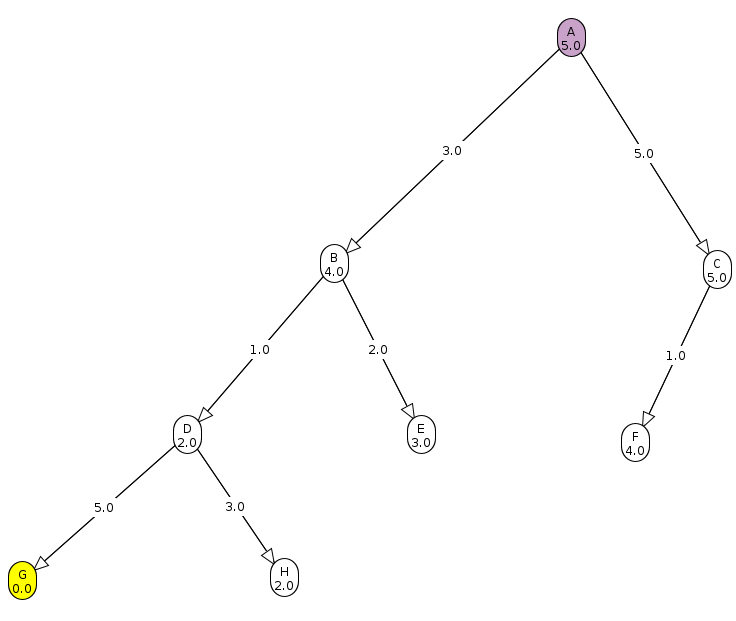
\includegraphics[width = \textwidth]{./1a.png}
    \caption{the solution node is a leaf node}
    \label{fig:1a}
\end{figure}

As can be seen in figure~\ref{fig:1a}, DFS is more efficient than BFS since it is a leaf node. Since it is on the left-most side of the graph, there is no need for DFS to expand nodes C, E and F. Thus BFS requires us to expand seven nodes while we only need to expand four nodes for DFS. 

\subsection*{b. Give a graph where BFS is much better than DFS}

\begin{figure}[H]
\centering
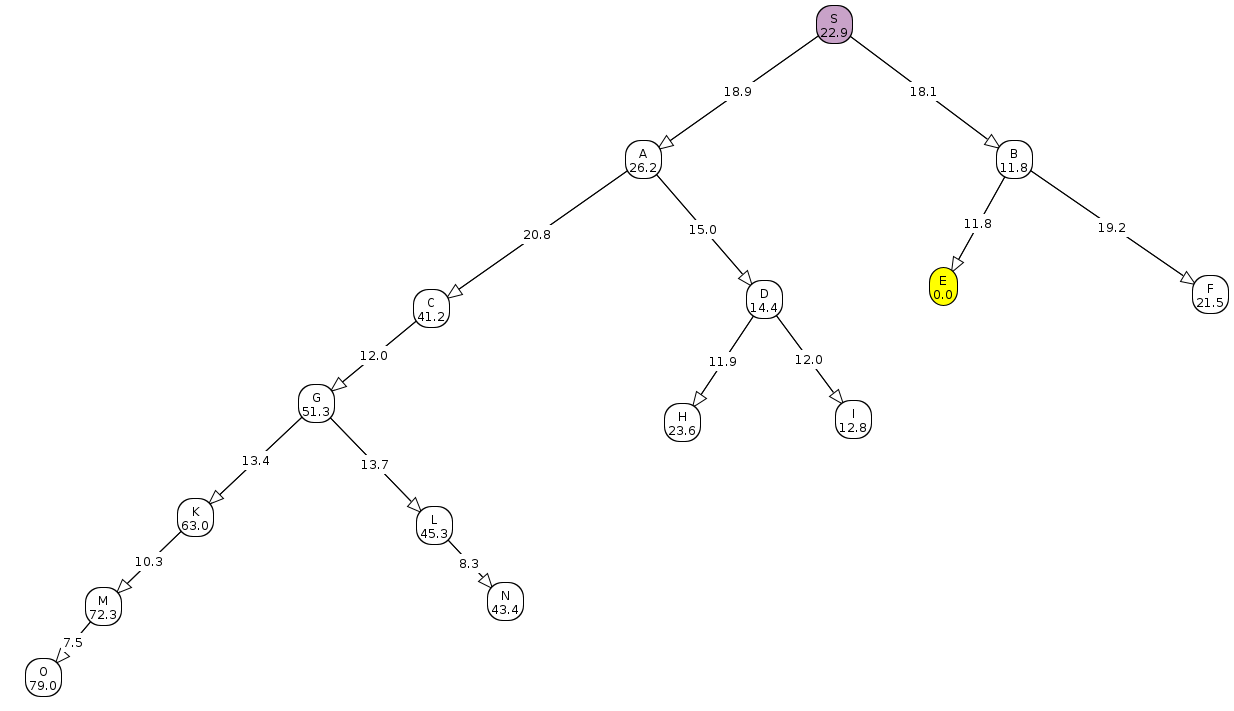
\includegraphics[width = \textwidth]{./1b.png}
    \caption{the solution node is a leaf node of depth 2}
    \label{fig:1b}
\end{figure}

As can be seen in figure~\ref{fig:1b}, BFS is more efficient than DFS since it is a leaf node. Since it is on the right side of the graph and is quite shallow, BFS would only expand nodes A, B, C, D, and E while DFS would expand A, B, C, G and etc. Thus, BFS has us expanding only six nodes while DFS would require us to expand 14 nodes.

\subsection*{c. Give a graph where A* search is more efficient than either BFS or DFS}

\begin{figure}[H]
\centering
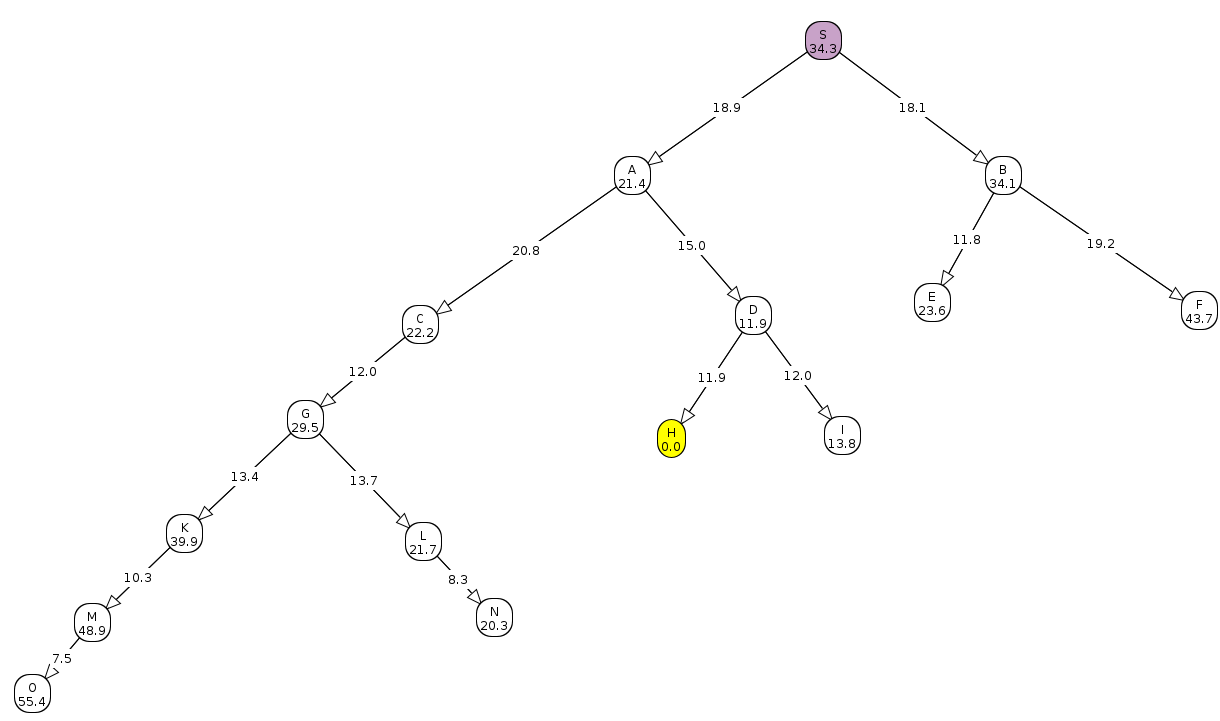
\includegraphics[width = \textwidth]{./1c.png}
    \caption{the heuristic function is accurate}
    \label{fig:1c}
\end{figure}

Since the efficiency of A* Search depends largely on the accuracy of the heuristic function, having a heuristic function that accurately predicts the distance to the goal allows for a very efficient search algorithm. In~\ref{fig:1c}, we have a very accurate heuristic and this allows us to only expand four nodes in order to reach node H using A* Search. This is in contrast to DFS which requires to expand 11 nodes and BFS which requires us to expand 9 nodes.  

\subsection*{d. Give a graph where DFS and BFS are more efficient than A* Search}

\begin{figure}[H]
\centering
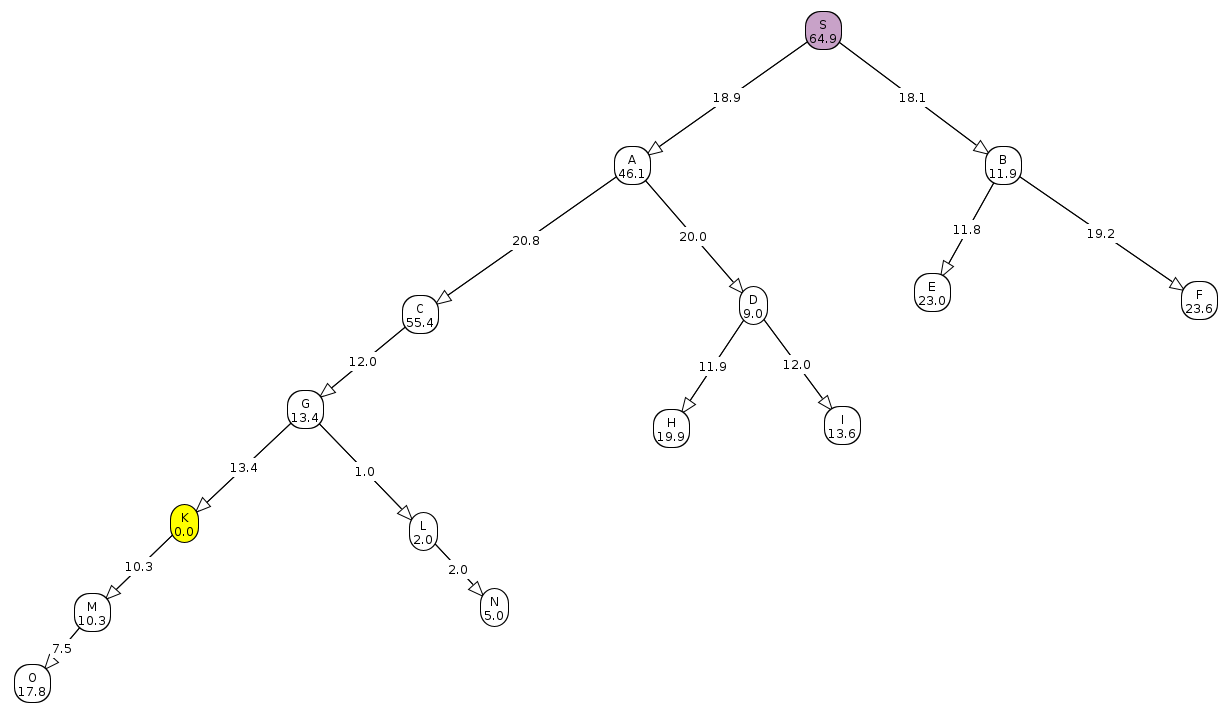
\includegraphics[width = \textwidth]{./1d.png}
\caption{the heuristic function is not accurate}
\label{fig:1d}
\end{figure}

In~\ref{fig:1d}, it can be seen that the heuristic function is inaccurate. This results in A* Search expanding 13 nodes in order to reach the goal state. However, since the goal node is deep, DFS results in a more efficient search since it only needs to expand five nodes. BFS also results in a more efficient search since there are only 11 nodes expanded. 

\newpage
\section*{Question Two}

\subsection*{a. What is the effect of reducing $h(n)$ when $h(n)$ is already an underestimate}

When $h(n)$ is an underestimate, this means that all of the nodes are mistakenly assumed to be closer to the goal than they actually are. By further reducing $h(n)$, this means that the effect of the heuristic function is even more reduced which makes the heuristic even less accurate. The evaluation function $f(n)$ used by A* search is a combination of the actual cost $g(n)$ to reach node $n$ as well as the heuristic function $h(n)$. \\

\noindent By reducing the heuristic function when it is already an underestimate, this means that the evaluation function, $f(n)$ is affected by $g(n)$ even more. This moves the A* search algorithm closer to that of an uninformed Uniform Cost Search the more we reduce $h(n)$. \\

\noindent Thus, we can conjecture that the accuracy of A* will not be affected. This is because both Uniform-Cost Search (a special case of A* search when $h(n)$ is 0) and A* are both complete and optimal. \\

\noindent However, its efficiency will be reduced. This is because an informed search is meant to speed up the search algorithm by means of a heuristic function. Thus, by reducing the effect of the heuristic function. While both Uniform-Cost Search and A* Search has an asymptotic time complexity. A* Search is usually more efficient in terms of run-time speed. Thus, reducing $h(n)$ when it is already an underestimate would increase the run-time of the search algorithm in most cases since more nodes may be expanded (or the same number of nodes). 

\subsection*{b. How does A* perform when $h(n)$ is the exact distance from $n$ to a goal}

\begin{figure}[H]
\centering
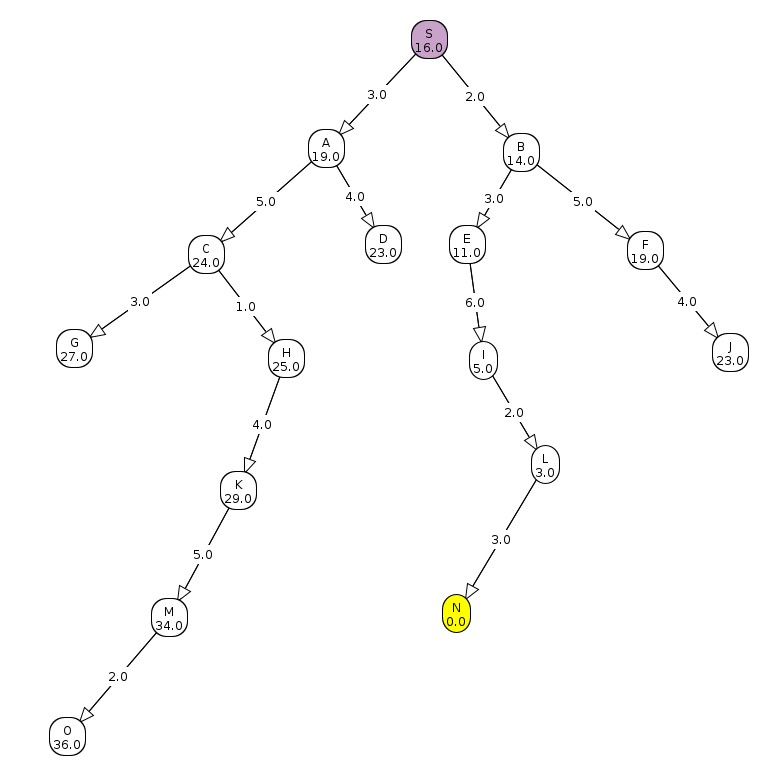
\includegraphics[width = \textwidth]{./2b.png}
\caption{Exact heuristic function}
\label{fig:2b}
\end{figure}

Given $f(n) = g(n) + h(n)$ and $h(n)$ is the exact distance to the goal. This means that the search algorithm has a complete knowledge of the graph. Thus, it would only expand nodes that is in the optimal path to the goal node.

\subsection*{c. What happens if $h(n)$ is not an underestimate}

When $h(n)$ is not an underestimate, it is either an exact distance or an over estimate. If it is the exact distance, the matter has been discussed in part b of this question. If the heuristic function is an overestimate, this means that the distance to the goal is shorter than the heuristic function estimated it to be. Thus, this would mean that in a lot of cases, a non-optimal path is obtained instead of the optimal path. This is because $g(n)$, the actual information we have from the past is overshadowed by the increase in $h(n)$. Thus, this means that the algorithm is likely to explore a suboptimal path instead since it may perceive a node in the optimal path to be further away from the goal node than it actually is. \\

\noindent However, we can also see that if $h(n)$ is an overestimate, this means A* Search becomes closer to a greedy best-first search. This is because the evaluation function plays a less important role when $h(n)$ becomes a lot larger than $g(n)$. Thus, this may actually increase the efficiency of the algorithm since a solution will be given faster than normal. However, just like in Greedy search, it is likely that the path given won't be the optimal path. Thus, by overestimating $h(n)$, in a majority of cases, it becomes more like a greedy search and hence would return a solution quicker albeit not an optimal one. 

\begin{figure}[H]
\centering
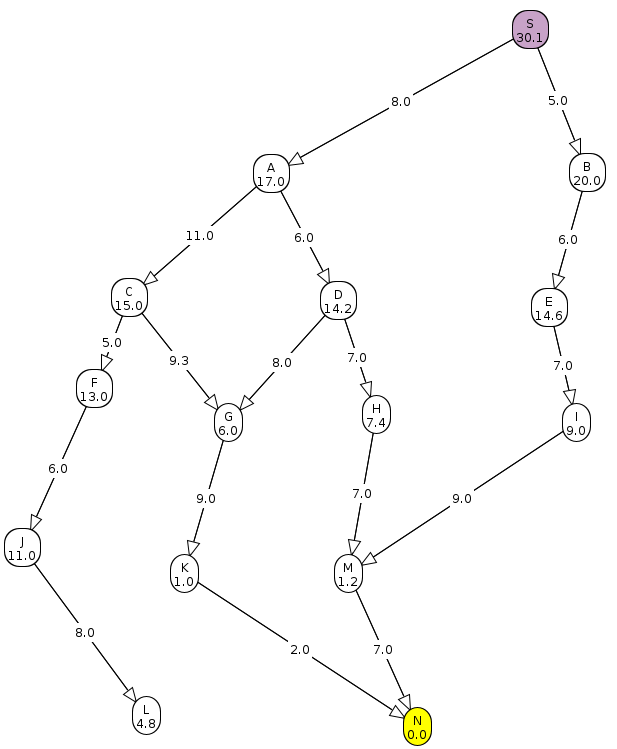
\includegraphics[width = \textwidth]{./underestimate.png}
\caption{underestimated heuristic function}
\label{fig:2c-underestimate}
\end{figure}

\noindent Given figure~\ref{fig:2c-underestimate}, we can see that the A* Search algorithm returns to us the optimal path to the goal state. However, in doing so, it expanded 10 nodes [S, A, B, D, E, I, G, M, K, N]. \\

\begin{figure}[H]
\centering
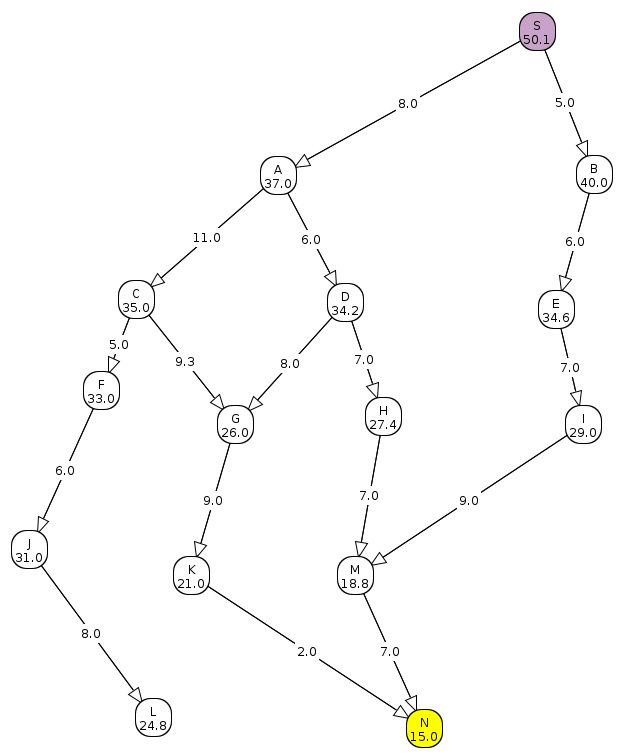
\includegraphics[width = \textwidth]{./overestimate.png}
\caption{overestimated heuristic function}
\label{fig:2c-overestimate}
\end{figure}

\noindent Since N is the goal state, the value for $h(n)$ will be 0 there. Thus, we can see in figure~\ref{fig:2c-overestimate} that by overestimating we only need to expand 7 nodes in order to get a solution to the path [S, A, B, E, I, M, N]. This is because the algorithm now behaves more like a greedy search and hence it returns a path quicker but this path is not the optimal path. 

\end{document}
